\chapter{Asking Wealthy Americans How They Got Rich! (Scottsdale)}

This chapter records a field lecture in commercial mechanics. There is no blackboard, yet the variables are remarkably stable: prior scarcity, ownership share, revenue, firm value, debt, liquidity, sales structure, and the discipline required to keep a growing business alive. The host does not begin with a theorem and then prove it. He asks the same small battery of questions in public --- Were you ever broke? What do you do? How much did you make? What was the low point? How did you scale? --- and the answers gradually assemble a theory of how wealth is built, financed, protected, and sometimes lost.

\section{Montage, Setting, and Method}

The episode begins with a compressed montage: a Ferrari, a claim of entrepreneurship, a former military life, business buying and selling, a reported \$11 million year, and the refrain of focus and discipline. We should read this opening as a preview reel, not as a continuous proof. Its function is to set the scale of the inquiry before the method is formally stated.

Only then does the host name the setting. We are in Scottsdale, at Fashion Square, one of the richest cities in the country, and the plan is simple: walk the place, find people who have actually built wealth, and ask direct questions until the mechanisms begin to appear. That structure matters. The lecture is not organized by textbook topic but by repeated public probing. Each interview begins with a familiar entry point and then, if the speaker stays, opens into some combination of revenue, ownership, financing, scale, and personal cost.

\begin{definition}
For the notes we write $R$ for annual revenue, $\operatorname{ARR}$ for annual recurring revenue, $V$ for company value, $W$ for owner net worth, $\alpha$ for founder ownership share, $D$ for bank debt, $E$ for outside equity, and $C_t$ for cash on hand at time $t$. These symbols are editorial bookkeeping devices, introduced only to keep the lecture's quantitative claims from collapsing into one another.
\end{definition}

\begin{table}[h]
\centering
\begin{tabular}{|p{3.1cm}|p{4.3cm}|p{5.8cm}|}
\hline
Interviewee & Reported magnitude & Reading \\
\hline
Fitness entrepreneur & $\operatorname{ARR} > 20\,\mathrm{M}$, target $R > 100\,\mathrm{M}/\mathrm{yr}$ & Online fitness and nutrition business, only three years old, already thinking in recurring revenue and in the next order of scale. \\
\hline
Healthcare founder & $R \approx 100\,\mathrm{M}/\mathrm{yr}$, $V \approx 1\,\mathrm{B}$, $W \in [500,700]\,\mathrm{M}$ & Founder and CEO in healthcare, claiming full ownership and no outside capital. \\
\hline
Industrial distributor & $R \approx 250\,\mathrm{M}/\mathrm{yr}$ in good years & Long-horizon industrial business built out of family apprenticeship, hiring, financing, and implementation. \\
\hline
Ex-military operator & $R_{\max} \approx 11\,\mathrm{M}/\mathrm{yr}$ & Business buying and selling, then work in venture capital, private equity, and investment banking. \\
\hline
\end{tabular}
\caption{Reported magnitudes that organize the later interviews. When the montage and the fuller interview disagree in clarity, the fuller interview takes precedence.}
\end{table}

\begin{remark}
The lecture's numbers are conversational and self-reported. We should therefore preserve them faithfully while resisting the temptation to squeeze from them more precision than the transcript can support.
\end{remark}

\section{Access Is Part of the Story}

Before the lecture yields a real business case, it gives us something else: refusal. A few people disengage, a few keep walking, one does not want social media at all, and the host is forced to keep resetting the interaction. That sequence is not dead air. It establishes the first principle of the episode: wealth protects time. The difficulty of getting an answer is itself part of the argument.

The host says this out loud. In a rich city it is hard to get access to wealthy people because they understand the value of their time and are always moving. He then makes a promise not to leave until he has delivered something substantial. This is the point at which the lecture earns its transition. We have seen the cost of access; now we are ready for the first sustained conversation.

\section{Ownership, Recovery, and Retained Upside}

The first full case is the healthcare founder. Here the lecture shifts from atmosphere to structure. We are told that the speaker has spent roughly twenty-four years in entrepreneurship, that a serious low point came when he gambled on the wrong staff and got burned, and that his superpower as an owner is communication: he talks to everybody on a regular basis. The details of the business follow. He is a retired doctor, now founder and CEO, and the company is in healthcare, providing comprehensive care for trauma patients: surgeries, scar revisions, site counseling, physical therapy, chiropractic care, and general medical management. The list matters because it shows breadth of service rather than a single narrow product.

The host then moves to the deeper question: where did the trajectory change? The founder says he did not come from money. As a child, even McDonald's felt like a treat. The family shift, he says, came from watching his father build custom homes as a hobby and noticing that the people in those neighborhoods did not simply have jobs. They owned something. This is the section's conceptual hinge. The lecture wants us to see that the decisive move is not merely toward a profession, but toward ownership of the economic machine.

\subsection{Question \& Answer}

\paragraph{Question.} How does one change a family's trajectory, and where does the initial capital come from?

\paragraph{Answer.} The answer has two layers. First, the model of success changes: one does not merely become a doctor, one tries to own the practice. Second, on the founder's own account, the capital structure is kept maximally concentrated. He says there were no banks, no investors, no private equity, no other owners. The lecture does not present this as a universal recipe. It presents it as a particular and very powerful configuration.

The bookkeeping distinction we need is the following:
\begin{align}
W &= \alpha V + A - L, \\
V_{\text{stake}} &= \alpha V.
\end{align}
Here $A$ stands for other personal assets and $L$ for liabilities or senior claims. The point is elementary but essential. Revenue $R$, company value $V$, and personal wealth $W$ are different objects. If ownership is highly concentrated, then changes in $V$ pass much more directly into the owner's balance sheet.

For this interview the transcript-backed simplification is
\begin{equation}
\alpha = 1,
\end{equation}
so the founder's direct claim on the enterprise is simply
\begin{equation}
V_{\text{stake}} \approx V.
\end{equation}
That is the clean reason the host cares so much about outside capital. If $E=0$ and $\alpha$ stays near one, then the upside is not being shared away.

We should be careful with the numbers. The founder reports roughly $100\,\mathrm{M}$ in annual revenue, says the company may be worth around $1\,\mathrm{B}$, and places his personal net worth somewhere between $500$ and $700\,\mathrm{M}$. These figures should be preserved as stated claims, not reverse-engineered into a precise capitalization model. The value of the notation is not false exactness. It is that it keeps the categories from blurring.

The host immediately compresses the lesson in his recap. Keep cash in the business. The claim is not mere thrift. If the owner keeps the whole upside, then retained liquidity becomes part of defending the very asset from which that upside is drawn. One bad month, says the host, can blow the cash and end the game. The lecture will return to this point later in a sharper form.

A final beat closes the case. The founder says he sacrificed heavily: he rarely saw the children wake up, rarely saw them go to bed, worked six days a week, and took Sunday for a nap. His wife says people joked that perhaps he had been hired for Facebook because they never saw him. So the section does not end with valuation. It ends with cost. Ownership and upside come tied to time spent elsewhere.

\section{Scaling Without Breaking the Firm}

The lecture then resets and finds a different kind of entrepreneur: younger business, faster rise, different sector, but the same underlying question. This speaker runs an online fitness and nutrition company, has been in business for only three years, reports more than $20\,\mathrm{M}$ in annual recurring revenue, and says explicitly that this is only the beginning.

The headline quantities are stated in the open:
\begin{equation}
\operatorname{ARR}_{\text{fitness}} > 20\,\mathrm{M}, \qquad
R_{\text{fitness,target}} > 100\,\mathrm{M}/\mathrm{yr}.
\end{equation}
The host, however, does not stop at the headline. He asks what really took the company from seven figures to eight. That is the right question. Once the lecture turns from wealth display to mechanism, scale must be decomposed rather than admired.

\subsection{Question \& Answer}

\paragraph{Question.} What actually takes a business from seven figures to eight?

\paragraph{Answer.} The answer arrives in an ordered chain. First, demand must be captured, which the speaker identifies as marketing and sales. But that only solves the front end. Once demand is converted into paying customers, a second difficulty appears: the business must fulfill the service without letting the client experience break. If growth outruns operations, then success at the level of demand creates failure at the level of delivery.

\begin{figure}[h]
\centering
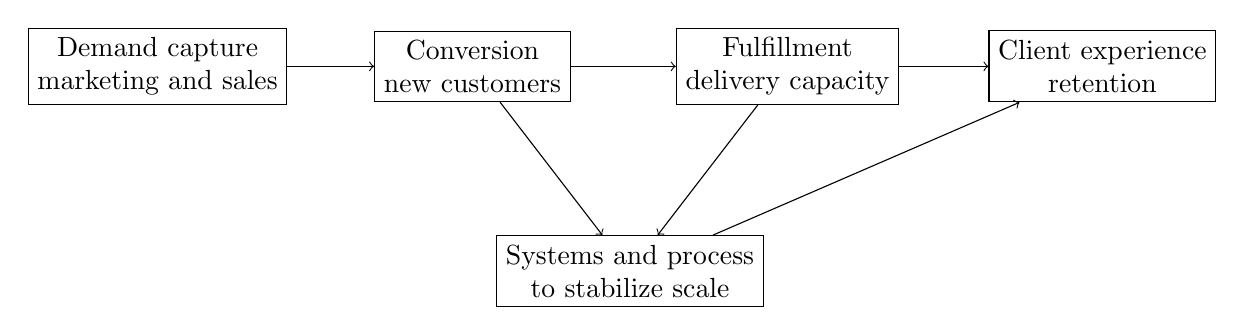
\begin{tikzpicture}
\node[draw, rectangle, align=center] (m) at (0,0) {Demand capture\\marketing and sales};
\node[draw, rectangle, align=center] (c) at (4,0) {Conversion\\new customers};
\node[draw, rectangle, align=center] (f) at (8,0) {Fulfillment\\delivery capacity};
\node[draw, rectangle, align=center] (x) at (12,0) {Client experience\\retention};
\node[draw, rectangle, align=center] (p) at (6,-2.6) {Systems and process\\to stabilize scale};
\draw[->] (m) -- (c);
\draw[->] (c) -- (f);
\draw[->] (f) -- (x);
\draw[->] (c) -- (p);
\draw[->] (f) -- (p);
\draw[->] (p) -- (x);
\end{tikzpicture}
\caption{A transcript-derived scaling chain. The lecture's operational point is that top-line growth must be matched by systems, process, and fulfillment capacity.}
\end{figure}

If we let $M$ denote demand capture, $F$ fulfillment capacity, and $X$ the quality of the client experience, then the note-worthy relation is not subtle:
\begin{equation}
M \uparrow \quad \text{while} \quad F \not\uparrow
\qquad \Longrightarrow \qquad
X \downarrow.
\end{equation}
This is not an exact numerical law; it is a structural warning. Marketing and sales can work perfectly and still create a problem if operations lag behind them.

That is why the speaker immediately adds a second requirement: someone with real operational experience must build systems and process. The business becomes a coordinated machine, not merely a demand engine. In the lecture's own rhythm, this is the transition from enthusiasm to engineering.

From here the speaker broadens the lesson into self-investment. The best financial advice he received, he says, was to bet on himself. There was a period when he earned only \$19,000 a year, but mentally he already understood himself in richer terms. We should not misread this as empty positive thinking. Within the logic of the lecture, it is a claim about state variables. Present earnings are not the entire state. Skill, capacity, confidence, and the willingness to reinvest in oneself are forward variables that later show up in revenue and value.

The host pushes on age and time horizon. The entrepreneur says he became a millionaire only at forty, and therefore insists that it is never too late. He then gives the backward-facing advice that completes the section: do not care so much what others think; believe in yourself; become unapologetic about who you are. In other words, after the lecture has analyzed the scaling mechanism, it turns to the internal condition that sustains it.

A brief promotional interlude follows in the episode, but it does not alter the conceptual thread. When the lecture resumes, it asks the same questions in a more mature business setting.

\section{Implementation, Financing, and Sales Structure}

The industrial distributor provides the long-horizon counterpart to the fast-scaling fitness company. The speaker comes from a family business background, worked in his father's business through high school and college, and then helped start a company in the early 1980s. The business is described as a small distributorship in industrial selling, and in the good years it reached about $250\,\mathrm{M}$ in revenue. The temporal scale is completely different from the prior case. We are no longer watching a three-year sprint; we are watching the accumulation of a commercial system over decades.

\subsection{Question \& Answer}

\paragraph{Question.} What matters more: product or distribution?

\paragraph{Answer.} The lecture sets up this binary only to refuse it. The interviewee says that neither, taken by itself, is decisive. Products may be acceptable. Distribution may exist. Yet the business can still fail. The controlling variable is implementation: how the plan is actually carried out.

This is the right answer in the context of the episode because it blocks a common shortcut. One would like a single magic noun --- product, distribution, sales, capital --- to explain the whole business. The lecture repeatedly denies us that shortcut. It asks for mechanisms instead.

The speaker then unfolds the mechanism. To scale from eight figures to nine one must get the right people on the bus. Then come business plan, financing, and partners. Financing receives a particularly sober treatment. Yes, he used debt, but banks do not make startup borrowing easy. Unless one already has money, the banks do not want to lend it. That is not a side comment. It is the lecture's institutional reminder that capital access itself is uneven.

\begin{table}[h]
\centering
\begin{tabular}{|p{3.0cm}|p{2.3cm}|p{2.3cm}|p{5.4cm}|}
\hline
Case & Outside equity $E$ & Bank debt $D$ & Main lesson \\
\hline
Healthcare founder & $E=0$ as claimed & $D=0$ as claimed & Concentrated ownership preserves upside, but then retained cash becomes vital. \\
\hline
Industrial distributor & not emphasized & used, but difficult to obtain & Banks lend more easily to insiders than to those still trying to get started. \\
\hline
Ex-military operator & PE/VC/IB setting & market-facing & Sophisticated finance changes access, not the underlying need for liquidity. \\
\hline
\end{tabular}
\caption{A transcript-derived comparison of capital environments across the lecture's main cases.}
\end{table}

The section's second important definition concerns sales itself.

\begin{definition}
A hunter looks for new customers and new business. A farmer grows business inside existing accounts. A durable sales organization needs both roles.
\end{definition}

The corresponding schematic identity is
\begin{equation}
S_{\text{total}} = S_{\text{hunter}} + S_{\text{farmer}}.
\end{equation}
Again, the point is not accounting precision. The point is to preserve the division the speaker insists on. One part of the organization acquires. Another part deepens and protects what has already been acquired.

The interview then shifts, almost without warning, from firm mechanics to social diagnosis. The host asks whose generation works harder. The answer comes back in a contrastive form: once it was ``I earn,'' now too often it is ``I deserve.'' Whether we accept the complaint in full is less important than seeing its structural role. The lecture has moved from implementation in business to implementation in character. It is the same broad variable of discipline, now expressed in moral rather than financial language.

\section{Cash Flow, Contracts, and Leadership Under Pressure}

After a somewhat noisy transition, the final major case comes into focus. This speaker says he was broke in the military, then began buying and selling businesses, later moved overseas, ran aviation in Africa and construction in South America, and now works in the world of venture capital, private equity, and investment banking. The lecture has now accumulated stories about ownership, scale, implementation, and discipline. At this point it asks for the unifying constraint.

The speaker supplies it immediately. Eight out of ten businesses, he says, do not make it past five years. What is the most common mistake? Cash flow.

\subsection{Question \& Answer}

\paragraph{Question.} What is the most common mistake that prevents businesses from surviving?

\paragraph{Answer.} Cash flow. The speaker says it without hesitation and then sharpens it: revenue is excellent, but cash flow is what keeps the doors open.

The clean update rule is the plain bookkeeping identity
\begin{equation}
C_{t+1} = C_t + I_t - O_t,
\end{equation}
where $C_t$ is cash on hand at time $t$, $I_t$ cash inflows, and $O_t$ cash outflows. The speaker's practical recommendation is to build an eighteen-month cash-flow model, so we write
\begin{equation}
H = 18\,\mathrm{months}.
\end{equation}
The survival condition is then not a single annual number but a path condition:
\begin{equation}
C_t > 0 \qquad \text{for all } t \in [0,H].
\end{equation}
If at some point monthly obligations exceed opening cash plus incoming cash,
\begin{equation}
O_t > C_t + I_t,
\end{equation}
then the update rule gives
\begin{equation}
C_{t+1} < 0.
\end{equation}
That is the lecture's harshest reduction. A business can look healthy in the language of revenue and still fail in the language of liquidity.

The logic is simple enough to write as a short derivation:
\begin{enumerate}
\item Put the firm on a monthly grid $t=0,1,\dots,H$.
\item Update cash by $C_{t+1}=C_t+I_t-O_t$.
\item Demand that $C_t$ remain positive over the whole forecast window.
\item Conclude that business survival is a path condition on liquidity rather than a slogan about top-line growth.
\end{enumerate}

This final case then fans outward into the rest of the episode's vocabulary. Focus matters so much, he says, that there is no life balance while the work is underway. Good financial advice becomes contractual advice: nothing is real until there is a contract. Good negotiation advice becomes restraint: once the sale is made, stop talking. Good sales advice becomes role clarity: he is not the sales guy. His strength is leadership and motivation. Military experience enters not as decoration but as transferable structure: special operations, Green Beret discipline, and the ability to move that training into business.

The section ends, as the lecture itself does, by returning to the older refrain. At sixty the key words are still focus and discipline. The backward-facing advice to the twenty-year-old self is not a trick or a tactic. It is: stay in the fight.

\section{Summary}

The lecture gives us a sequence of commercial invariants rather than a single doctrine. First, wealth is repeatedly traced back to ownership. If upside is retained, then firm value matters to personal wealth in a direct way. Second, scale is shown to be a two-stage problem: demand capture first, then fulfillment and process, without which client experience breaks. Third, the lecture dissolves false binaries --- product versus distribution, sales versus leadership, revenue versus survival --- by replacing them with mechanisms. Fourth, cash flow emerges as the final gatekeeper. Revenue can impress. Liquidity decides.

What remains after the interviews are compressed is a consistent operating ethic: communicate, own when possible, keep cash inside the business when fragility is high, build systems before growth outruns them, distinguish acquisition from account development, respect contracts, know your role, and stay disciplined long enough for the numbers to mean something. The lecture arrives there not by abstraction alone, but by letting the same questions pass through several very different lives until the pattern is visible.